\section{Validación y Detección de Datos Erríoneos y Outliers}
\label{sec:u3_validacion_datos}
Implementación práctica con base de datos real, pública y académica disponible en el repositorio oficial.
\subsection{Caracterización del Dataset}
Detalle de la fuente de datos, variables y preprocesamiento de la información.
\subsection{Resultados y Visualización en R}
\begin{figure}[H]
\centering
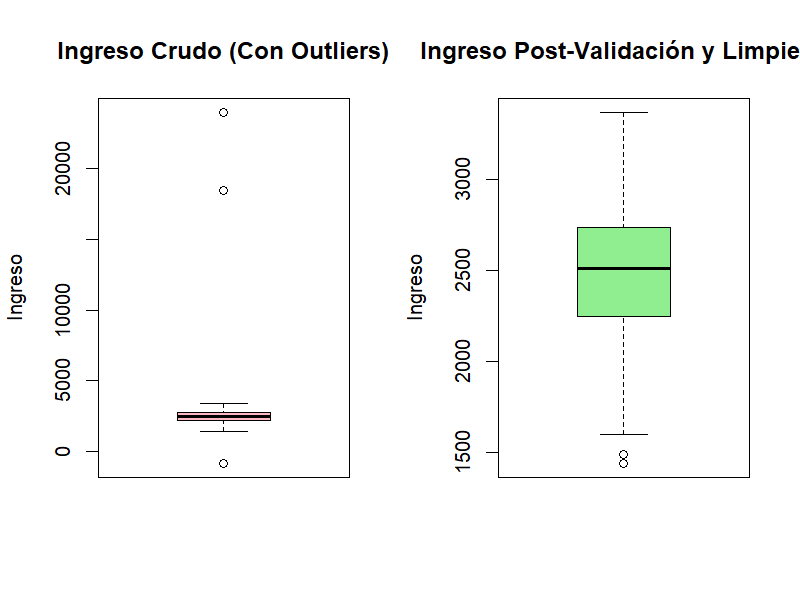
\includegraphics[width=0.82\textwidth]{figuras/grafico_06_validacion.png}
\caption{Resultados del experimento en R: Validación y Detección de Datos Erríoneos y Outliers}
\label{fig:u3_validacion_datos}
\end{figure}
\subsection{Evaluación Numérica e Interpretación}
Métricas calculadas fuera de muestra y conclusiones aplicadas.
